\documentclass[10pt,twocolumn]{article} 
\usepackage{simpleConference}
\usepackage{times}
\usepackage{graphicx}
\usepackage{amssymb}
\usepackage{url,hyperref}
\usepackage{xcolor}
\usepackage{mdframed}

\begin{document}

\title{CS670 Project Proposal\\Online Lockstep Behavior Detection}

\author{
Team Name: \textbf{End of Fraud}\\[2ex]
Team Members \small{(alphabetically ordered)}:\\[1ex]
Majid Alfifi, Parisa Kaghazgaran,  Xing Zhao
}

\maketitle
%\thispagestyle{empty}

%\begin{abstract}
%   This is a simple sample of a document created using \LaTeX
%   (specifically pdflatex)
%   that includes a figure from the Vergil visual editor for Ptolemy II
%   that was created by printing to the Acrobat Distiller to get a PDF file.
%   It also illustrates a simple two-column conference paper style,
%   and use of bibtex to handle bibligraphies.
%\end{abstract}
%

\section{Introduction}
 
% An article style is separated into sections and subsections with 
%   markup such as this.  Use \section*{Principles} for unnumbered sections.

\begin{figure}[!b]
%\begin{mdframed}
  \begin{center}
    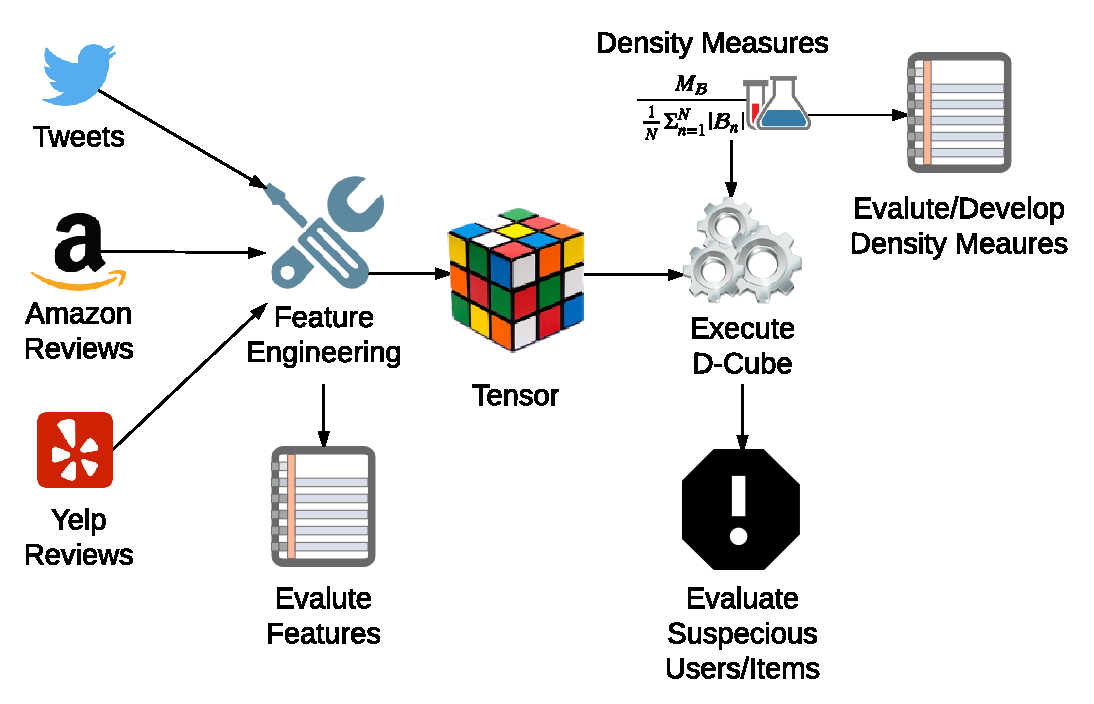
\includegraphics[width=3.5in]{figure.pdf}
  \end{center}
%\end{mdframed}
  \caption{\small Figure caption. To get a figure to span two
      columns, use the environment figure* rather than figure.}
  \label{fig:process}

\end{figure}

How can we detect if a politician has purchased fake followers on Twitter or if a product's reviews on Amazon are not genuine?

A common method has been to represent \emph{users} and \emph{items} as a matrix where in the simplest case a cell can take on a binary value of 1 if there is a relationship between the corresponding user and item or 0 otherwise. The problem can then be transformed to finding dense regions in this matrix \cite{hooi2016fraudar}. Moreover, this method has been lately extended from matrix to tensor representation to incorporate more dimensions from the domain such as timestamp, Twitter followers count, or number of stars of an Amazon product along with a scalable MapReduce-based implementation \textbf{D-Cube} [2]. Extraordinary dense blocks in the tensor correspond to groups of users with lockstep behaviors both in the items they relate to and along the additional dimensions (for example, multiple users reviewing the same products at the exact same time). 



\section{Project Goals}

As illustrated in Figure \ref{fig:process}, we intend to use an existing MapReduce-based implementation of the D-Cube algorithm\footnote{\href{https://github.com/kijungs/dcube}{https://github.com/kijungs/dcube}} (Section 3.3 in \cite{shin2017d}) on our own datasets with two main goals:
\begin{enumerate}
	\item \textbf{Feature engineering}: we will explore the effectiveness of different dimensions in each of our datasets in detecting fraudulent lockstep behavior; hopefully informing our own research.
	\item \textbf{Empirical study of density measures}: we aim to experiment and build on several density measures defined in \cite{shin2017d} (Section 2.2) and previously founded in \cite{jiang2015general} and potentially propose our own flexible density measures that take into account weights of different features in different datasets. For example, In Amazon dataset, is the temporal dimension more informative than product rating?
\end{enumerate}

\section{Datasets}
\begin{itemize}
\item \textbf{Twitter dataset}: 9 billion tweets of which 2 billion are from eventually suspended users.

\emph{Question:} Can we identify tweets/users tampering with hashtags in efforts to promote/undermine discussions in those hashtags? How do those suspicious tweets temporally differ from ordinary tweets (timestamp dimension)? Can we identify users hired to attack other users by continuously replying to their tweets casting doubt on their cause? etc. 
\item \textbf{Amazon dataset}: {\color{red} Parisa please add description here.} 

\emph{Question:} Can we find the hidden relation among reviewers in Amazon who aim to promote a product by writing fake reviews using additional dimensions such as temporal, rating and so on.  
\item Yelp dataset?: ... {\color{red}Xing please choose your dataset and what questions you want to answer} 
\end{itemize}




%The paper [2] defines several density measures appropriate for anomaly detection (Section 2.2). We aim to build on those functions and propose a flexible density measure which gives different weights to different features (e.g., In Amazon temporal features are more informative than rating).  
 
\section{Tools/Resources}
In addition to all the tools and methods we learned in the course, we will use a local Hadoop cluster to run the D-Cube algorithm.

\section{Project Outcome}

\begin{itemize}
	
	\item A set of users/items potentially participating in a lockstep behavior for each of the datasets under study.
	\item Evaluation of different dimensions. 
	\item Evaluation of different density measures.
	\item (Optional) New density measures that are more suitable to the nature of datasets we study.
\end{itemize}

\bibliographystyle{abbrv}
\bibliography{refs}
\end{document}
